\documentclass[11pt,a4paper,oneside]{report}
\usepackage{fontspec}
\usepackage{geometry}
\geometry{a4paper,top=2.6cm,bottom=2.6cm,left=2.6cm,right=2.4cm}
\usepackage{booktabs}
\usepackage{tabularx}
\usepackage{graphicx}
\usepackage{microtype}
\usepackage[table]{xcolor}
\usepackage{titlesec}
\usepackage{fancyhdr}
\usepackage{parskip}
\usepackage{caption}
\usepackage{float}
\usepackage{chngcntr}
% Figures are numbered straight through rather than per chapter, so the numbers match
% the captions in the markdown sources and the one reference to "Figure 6" in the text.
\counterwithout{figure}{chapter}

\definecolor{srhorange}{HTML}{E64415}
\definecolor{ink}{HTML}{1A1A1A}

% Interactive navigation, which is the point of this build: TOC entries, figure and
% section references, and the reader's sidebar all become links.
\usepackage[
  colorlinks=true, linkcolor=srhorange, citecolor=srhorange, urlcolor=srhorange,
  bookmarks=true, bookmarksopen=true, bookmarksnumbered=true,
  pdftitle={Building and Validating a Metal--Organic Framework Synthesis Knowledge Graph with Large Language Models}, pdfauthor={Devendra Singh Dhakad},
  pdfsubject={Case Study 2, SRH University of Applied Sciences Heidelberg}
]{hyperref}

\captionsetup{font=small,labelfont={bf,color=srhorange}}
\titleformat{\chapter}[display]
  {\normalfont\huge\bfseries\color{ink}}
  {\color{srhorange}\normalsize\bfseries\MakeUppercase{\chaptertitlename\ \thechapter}}
  {8pt}{\Huge}
\titlespacing*{\chapter}{0pt}{0pt}{24pt}
\titleformat{\section}{\normalfont\large\bfseries\color{ink}}{\color{srhorange}\thesection}{0.6em}{}

\pagestyle{fancy}
\fancyhf{}
\renewcommand{\headrulewidth}{0pt}
\fancyfoot[C]{\small\thepage}

\setlength{\emergencystretch}{3em}
\sloppy

\begin{document}

\begin{titlepage}
\centering

\includegraphics[width=4.2cm]{../assets/srh_logo.png}
\vspace{1.4cm}

{\color{srhorange}\rule{\linewidth}{1.2pt}}
\vspace{0.9cm}

{\LARGE\bfseries Building and Validating a Metal--Organic Framework Synthesis Knowledge Graph with Large Language Models\par}
\vspace{0.9cm}
{\color{srhorange}\rule{\linewidth}{1.2pt}}

\vspace{1.8cm}
{\large Case Study 2\par}
\vspace{2.2cm}

\begin{tabular}{rl}
\textbf{Author}         & Devendra Singh Dhakad \\[3pt]
\textbf{Matriculation}  & 100004684 \\[3pt]
\textbf{Programme}      & M.Sc. Data Science and Artificial Intelligence \\[3pt]
\textbf{Supervisor}     & Prof. Dr. Mehrdad Jalali \\[3pt]
\textbf{University}     & SRH University of Applied Sciences Heidelberg \\
\end{tabular}

\vfill
{\small Compiled from the chapter sources in \texttt{docs/report/}.\par}
\end{titlepage}

\tableofcontents
\clearpage


\chapter{Introduction}


\section{Motivation}

Metal-organic frameworks (MOFs) are porous crystalline materials assembled from metal nodes and organic linkers. Over 100,000 synthesised structures are recorded in the Cambridge Structural Database, and their applications span CO2 capture, gas storage and separation, catalysis, sensing and drug delivery. The knowledge of how any given MOF is actually made, which metal precursor and which organic linker, in which solvent, by which method, at which temperature and for how long, remains locked in the prose of tens of thousands of publications. Synthesis planning therefore still depends heavily on expert intuition and trial and error.

Large language models (LLMs) and knowledge graphs (KGs) together offer a route from that prose to a structured, queryable resource (Pan et al., 2024). Recent work demonstrates the approach at scale: Bai et al. (2025) built a knowledge graph of 2.53 million nodes for framework materials from more than 100,000 articles, and coupled it to a question-answering system. What that literature does not establish is reliability. How accurate are LLM-extracted synthesis records field by field? How do they compare with the text-mined databases the field already relies on, and with the rule-based systems that produced them? And what does an open-weight model deliver relative to a commercial API, at what cost?

\section{The gap this work addresses}

Three observations define the gap.

First, the existing LLM work on MOF text mining validates against small in-house test sets and uses commercial GPT models almost exclusively (Zheng et al., 2023; Shi et al., 2024; Lin et al., 2025). No published study reports per-field accuracy against both expert annotation and the established text-mined databases.

Second, the authors of DigiMOF, the largest openly available MOF synthesis database, state the problem directly. Writing about routes that papers imply through solvent and temperature rather than naming outright, they observe that such implicit routes "could be easily deduced by a reader but are challenging to extract using rule-based NLP" (Glasby et al., 2023). That is a precise, testable claim about where a language model should help and where it should not.

Third, the cost dimension of the open-weight question is unexamined, despite being the factor that decides whether a pipeline of this kind is reproducible by anyone without an institutional budget.

\section{Research questions}

\textbf{Main question.} How accurately and reliably can large language models extract complete MOF synthesis records, measured against expert annotation and domain-specific baselines?

\textbf{RQ1.} How does per-field extraction accuracy compare between LLMs and a rule-based baseline built from the same domain vocabulary?

\textbf{RQ2.} Which prompting strategy, among zero-shot, few-shot, schema-guided and chain-of-thought, is most reliable for each field of a synthesis record?

\textbf{RQ3.} Where and why do LLM extractions disagree with the DigiMOF and SynMOF reference databases?

\textbf{RQ4.} How do open-weight models compare with commercial APIs on per-field accuracy, cost and latency?

\textbf{RQ5.} Can the resulting knowledge graph answer aggregation queries across hundreds of papers?

\section{Contributions}

\begin{enumerate}
\item A reproducible, provenance-complete pipeline from open-access literature to a Neo4j knowledge graph, in which every entity carries a traceable link to the sentence and paper it came from, verified by query rather than asserted.
\item A hand-annotated gold standard of 100 MOF synthesis passages containing 138 triples, drawn by a seeded stratified sample that includes an unflagged control stratum, so the pre-filter's own error rate is measurable rather than assumed.
\item A per-field comparison of ten extractor configurations spanning a rule-based baseline, two commercial models and one open-weight model across four prompting strategies.
\item A pre-registered prediction about where language models should beat rules, recorded before any model was run and confirmed by the measurements.
\item An honest account of what the evaluation cannot show, including a field whose scores reflect annotation granularity rather than extraction quality, and two configurations removed rather than reported from partial data.
\end{enumerate}
\section{Structure of this report}

Chapter 2 reviews the state of the art. Chapter 3 sets out the methodology, including the ontology, corpus construction, annotation protocol and evaluation design. Chapter 4 describes the implementation. Chapter 5 presents the results. Chapter 6 discusses them. Chapter 7 states the limitations and threats to validity. Chapter 8 concludes.


\chapter{State of the Art}


Extracting synthesis knowledge from chemical literature has passed through three phases: rule-based systems built on hand-written grammars, transformer models pre-trained on domain text, and most recently large language models prompted rather than trained. This chapter follows that progression, then states precisely what remains unestablished, because the gap this work addresses is narrower than "language models have not been tried".

\section{Rule-based extraction and the databases it produced}

ChemDataExtractor (Swain \& Cole, 2016) established the template for automated chemical information extraction: a pipeline of tokenisation, chemical named-entity recognition and grammar-driven parsers producing structured records. Its strength is precision and auditability. A parser either matches or it does not, and the reason is inspectable.

That toolkit produced the two reference databases this work validates against. \textbf{DigiMOF} (Glasby et al., 2023) adapted ChemDataExtractor with MOF-specific parsers and applied it to 43,281 articles, yielding 15,501 MOFs and 52,680 synthesis-property records covering synthesis method, solvent, organic linker, metal precursor and topology. The published Supporting Information tabulates a larger structural set of 24,732 distinct CSD refcodes, which is the file Section 5.7 joins against; the two counts describe different artefacts of the same work rather than disagreeing. \textbf{SynMOF} (Luo et al., 2022) mined synthesis conditions for 983 MOFs, including metal source, linker, temperature, time, solvent and additives, and used them to train synthesis prediction models. It is distributed as an automatically extracted set of 983 records and a manually curated subset of 840; Section 5.7 uses the curated subset, and states which wherever a count appears.

The same approach has been applied beyond MOFs. Kim et al. (2017) mined oxide synthesis parameters, and Kononova et al. (2019) extracted 19,488 inorganic synthesis recipes into a codified action-graph schema. The latter is a useful precedent for the present work's ontology design, since it faced the same question of how finely to decompose a procedure into discrete steps and conditions.

\textbf{What this literature reports about its own limits} is the hinge of this chapter. Analysing their extracted data, the DigiMOF authors found more hydrothermal than solvothermal records, which they describe as surprising because solvothermal is the more common laboratory route. Their explanation is that many papers never name the route and instead imply it through solvent and temperature, and that such implicit routes "could be easily deduced by a reader but are challenging to extract using rule-based NLP" (Glasby et al., 2023).

That is a precise, falsifiable claim about where rule-based extraction fails and, by implication, where a system with broader language understanding should help. It is testable, and this work tests it.

\section{Domain-specific language models}

The second phase replaced hand-written grammars with pre-trained transformers. Weston et al. (2019) applied named-entity recognition and normalisation to 3.27 million materials abstracts. MatSciBERT (Gupta et al., 2022) showed that pre-training on materials text substantially outperforms general-purpose BERT on domain named-entity recognition, and Trewartha et al. (2022) quantified that advantage systematically. Tshitoyan et al. (2019) demonstrated that unsupervised embeddings trained on materials literature encode latent domain knowledge, to the point of anticipating later discoveries. Olivetti et al. (2020) survey the field as it stood before language models.

These systems improve entity recognition but share two constraints relevant here. They require labelled training data, and they operate at entity level rather than producing complete, linked records. Recognising that "DMF" is a solvent does not establish which synthesis used it.

\section{Large language models for chemical extraction}

The third phase prompts general-purpose models rather than training domain-specific ones. Wei et al. (2023) showed that decomposing extraction into a two-stage dialogue makes zero-shot information extraction competitive. Dagdelen et al. (2024) demonstrated that language models can emit structured JSON records combining entities and relations for materials tasks, and set out a human-in-the-loop annotation scheme. Polak and Morgan (2024) reported precision and recall above 90 percent on materials property extraction using conversational follow-up prompts with uncertainty filtering. Jablonka et al. (2024) showed that fine-tuned models match or exceed bespoke machine learning on chemistry prediction from small datasets.

Within MOF research specifically, Zheng et al. (2023) used prompt-engineered ChatGPT to mine synthesis parameters from 228 articles, feeding a synthesis-prediction model. Shi et al. (2024) showed that selecting few-shot demonstrations markedly improves MOF synthesis-condition extraction over zero-shot prompting, with roughly four examples sufficient. Lin et al. (2025) proposed a multi-agent framework dividing planning, extraction and validation across cooperating agents. Ansari and Moosavi (2024) and Yang et al. (2026) extend the agentic approach to autonomous dataset construction and to catalytic reaction data. Bae et al. (2025) survey the whole manual-to-rule-based-to-language-model transition in MOF text mining.

\textbf{Three properties recur across this body of work.} Validation is against small in-house test sets rather than against the established databases the field already uses. The models evaluated are almost exclusively commercial GPT variants. And cost is rarely reported at all, despite being the factor that decides whether a pipeline can be rerun by a group without an institutional budget.

\section{Language models and knowledge graphs}

Pan et al. (2024) provide the organising framework for combining language models with knowledge graphs, distinguishing knowledge-graph-enhanced models, model-enhanced knowledge graphs, and synergised systems, and identifying model-driven graph construction as an open problem.

That problem has since been addressed at scale. Bai et al. (2025) constructed a knowledge graph for framework materials from over 100,000 articles, producing 2.53 million nodes and 4.01 million relations covering synthesis, properties and applications, and coupled it to a question-answering system reporting 91.67 percent accuracy. Ye et al. (2024) built a comparable multidisciplinary materials graph and used it for cross-domain link prediction, and Yoshitake and Nagata (2025) describe a method for property-focused graph construction. Dreger et al. (2025) show that tables are a distinct, high-density extraction target that prose-oriented pipelines miss.

Retrieval-augmented generation (Lewis et al., 2020) and its graph-structured successor GraphRAG (Edge et al., 2024) establish why such graphs are useful downstream: grounding generation in retrieved structure improves factuality, and graph structure specifically helps on aggregation questions that span many documents.

Scale is therefore demonstrated. What these papers do not report is per-field extraction validity: how often each individual field of an extracted record is correct.

\section{Why validated MOF data matters downstream}

The value of accurate synthesis records is not confined to retrieval. Luo et al. (2022) train synthesis-prediction models directly on mined conditions, so extraction errors propagate into predictions. MOFGalaxyNet (Jalali et al., 2023) represents the MOF landscape as a network of linker and metal similarity and predicts guest accessibility using graph convolutional networks, an approach that depends on reliable structured descriptions of each framework. CoRE MOF (Chung et al., 2019) provides curated computation-ready structures, and MaScQA (Zaki et al., 2024) benchmarks language models' materials knowledge, finding strong overall performance alongside systematic conceptual failure modes.

Extraction quality is therefore an input to a chain of downstream work, which is what makes measuring it per field worth doing rather than reporting a single aggregate.

\section{The gap}

Bringing the three strands together:

\begin{enumerate}
\item \textbf{Rule-based systems} are precise and auditable, and their own authors identify implicit synthesis routes as their characteristic failure (Glasby et al., 2023).
\item \textbf{Language models} have been applied to MOF extraction repeatedly, but validated against small in-house sets, using commercial models almost exclusively, and rarely with cost reported.
\item \textbf{Knowledge graph construction} has been demonstrated at a scale of millions of nodes, without per-field validity being established.
\end{enumerate}
No published study evaluates language-model MOF synthesis extraction field by field against both expert annotation and a rule-based baseline built from the same domain vocabulary, while also reporting what each configuration costs and how an open-weight model compares.

This work occupies that gap. It is deliberately small in scale where the cited work is large, and correspondingly more careful about what each number means: a hand-annotated gold standard, a baseline built to succeed rather than to lose, per-field scores reported with their support counts, and an explicit account of what the evaluation cannot show.


\chapter{Methodology}


\section{Ontology}

The extraction target is defined by a MOF-specific ontology (v0.2) held in \texttt{configs/ontology.json}, which is the single source of truth for the type system. Nine entity types are defined: MOF, MetalPrecursor, OrganicLinker, Solvent, SynthesisMethod, Condition, Property, Application and Paper. Nine relations connect them:

\begin{center}
\small
\begin{tabular}{@{}lrr@{}}
\toprule
\textbf{Relation} & \textbf{From} & \textbf{To} \\
\midrule
USES\_PRECURSOR & MOF & MetalPrecursor \\
USES\_LINKER & MOF & OrganicLinker \\
SYNTHESIZED\_BY & MOF & SynthesisMethod \\
IN\_SOLVENT & SynthesisMethod & Solvent \\
AT\_CONDITION & SynthesisMethod & Condition \\
HAS\_PROPERTY & MOF & Property \\
MEASURED\_AT & Property & Condition \\
USED\_IN & MOF & Application \\
MENTIONED\_IN & any & Paper \\
\bottomrule
\end{tabular}
\end{center}
Two design decisions in this table matter later. Solvents and conditions attach to a synthesis method rather than directly to the MOF, so the method acts as a connector; this is what makes the object of those relations the substantive claim. And MENTIONED\_IN is never produced by an extractor: it is attached by the pipeline from passage metadata, so that provenance cannot be hallucinated.

The type literals in the extraction interface are checked against the ontology file by automated tests, so the two cannot drift apart silently.

\section{Corpus}

Papers were collected from the Europe PMC open-access subset, which exposes structured JATS full text with labelled sections. This was preferred over publisher scraping and PDF parsing because section labels are given rather than inferred, which the segmentation step depends on.

The query was \texttt{(metal-organic framework AND synthesis) AND OPEN\_ACCESS:y AND HAS\_FT:y AND IN\_EPMC:y}. The collected corpus is \textbf{399 papers and 20,582,200 characters}, every one carrying a DOI. Licences are 299 CC BY, 56 CC BY-NC-ND, 43 CC BY-NC and 2 unrecognised, the last of which are excluded from redistribution pending verification.

Publisher distribution by DOI prefix is RSC 107, MDPI 78, ACS 75, Nature 40, Wiley 40, Elsevier 11 and a long tail. This matters for RQ3: RSC, ACS and Wiley are the publishers DigiMOF drew from, so an open-access Europe PMC corpus does overlap the reference database's source population.

One paper was returned twice by the search API across cursor pages. Deduplication by PMCID and DOI is applied at collection, because passage identifiers are derived deterministically from the paper identifier and a duplicate paper would otherwise produce colliding passage identifiers in the gold standard.

\section{Segmentation}

The unit of extraction is the synthesis paragraph, not the paper. Papers run 20,000 to 50,000 characters and most of that text contains no recipe, so passing whole papers to an extractor would be both expensive and noisy.

Sections are split into paragraphs with character offsets preserved, short fragments merged into neighbours and long paragraphs split. Each passage receives a stable, deterministic identifier derived from the paper identifier, section name, section occurrence and index, so that the gold standard's references survive a corpus rebuild.

Each passage is scored for synthesis content by a transparent weighted rule set whose weights are module-level constants and sum to 1.0, with saturation caps so that one repeated word cannot carry a passage. The signals are section-title cues, method words, quantity and unit patterns, apparatus terms, MOF solvents and procedure verbs. A learned filter was rejected deliberately: it would need labelled data that this project spends on the gold standard instead, and its decisions could not be recomputed by a reader.

Segmentation produces \textbf{22,086 passages}, of which \textbf{794 across 224 papers} are flagged as synthesis at the chosen threshold of 0.45, with a mean length of 931 characters.

The threshold is a declared choice, not an accident. Its sensitivity is:

\begin{center}
\small
\begin{tabular}{@{}lrr@{}}
\toprule
\textbf{Cutoff} & \textbf{Passages} & \textbf{Papers} \\
\midrule
0.25 & 2,369 & 325 \\
0.35 & 1,369 & 267 \\
\textbf{0.45} & \textbf{794} & \textbf{224} \\
0.55 & 485 & 190 \\
0.65 & 268 & 149 \\
\bottomrule
\end{tabular}
\end{center}

\begin{figure}[H]
\centering
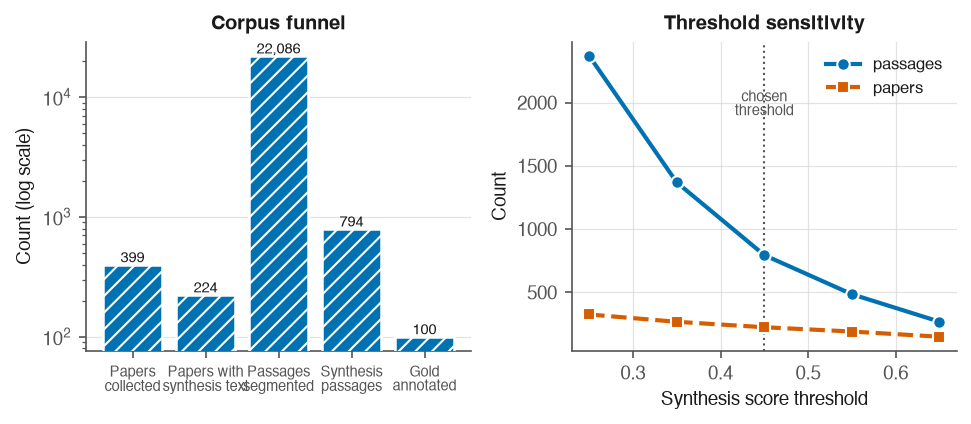
\includegraphics[width=\linewidth]{figures/fig5_corpus_and_threshold.pdf}
\caption{Left, the corpus funnel from collection to the gold standard, on a log scale because each stage is roughly an order of magnitude smaller than the last. Right, the same threshold sensitivity as the table, shown as a curve so the chosen cutoff of 0.45 can be seen sitting on the shoulder of the curve rather than at an arbitrary point on a steep slope.}
\label{fig:fig5_corpus_and_threshold}
\end{figure}

\section{Gold standard}

\textbf{Provenance of the annotations.} The gold standard is the instrument against which the language models are measured, so it was produced by the author by hand. Pre-filling it with model output, even from a model not under test, would make the evaluation circular and is the single shortcut this project could not take.

\textbf{Sampling.} The worklist is 100 passages drawn with a fixed seed: 90 from the synthesis-flagged pool and \textbf{10 control passages that the pre-filter did not flag}. The control stratum exists so that the pre-filter's own miss rate is measurable; without it, every recall figure reported here would be silently conditional on an unvalidated heuristic. The two strata are interleaved rather than blocked so that annotator fatigue does not fall entirely on one of them.

The sample size was reduced from the 150 to 200 stated in the exposé, on 2026-08-31, because annotator hours are the binding constraint and the submission date is fixed. The cost is precision, reported as wider confidence intervals and reduced support for rare relations. The stratification, the seed and the control stratum were preserved, because those are what make the evaluation reproducible.

\textbf{Tooling.} Annotation used a purpose-built interface in which the relation is chosen first and the subject and object types are then constrained to that relation's legal endpoints, so an ontology-invalid triple cannot be created. Work is autosaved after every action.

\textbf{Result.} 100 records containing \textbf{138 triples}. 32 passages contain synthesis records and 68 do not. Per-relation support is:

\begin{center}
\small
\begin{tabularx}{\linewidth}{@{}Xr@{}}
\toprule
\textbf{Relation} & \textbf{Support} \\
\midrule
USES\_PRECURSOR & 39 \\
IN\_SOLVENT & 34 \\
AT\_CONDITION & 34 \\
USES\_LINKER & 30 \\
SYNTHESIZED\_BY & 1 \\
HAS\_PROPERTY, MEASURED\_AT, USED\_IN & 0 \\
\bottomrule
\end{tabularx}
\end{center}
Only the first four relations carry enough support to support a conclusion. The scarcity of the others is itself a finding about where information sits in a paper: properties and applications are rarely stated inside a synthesis paragraph.

\section{Extractors}

All extractors implement one interface and return the same triple shape, so that every strategy is evaluated on identical terms. The interface forbids raising: a failure is recorded in the result rather than aborting a batch.

\textbf{Rule-based baseline.} A dictionary and regular-expression system whose vocabulary is derived from the MOF-adapted ChemDataExtractor parsers used to build DigiMOF and from inspection of the corpus. It was built to work rather than to lose, because a weak baseline would make every reported improvement meaningless. It attempts implicit synthesis routes rather than skipping them, emitting an inferred route at low confidence with a null span so that explicit and inferred routes can be scored separately.

\textbf{Language models.} Four prompting strategies (zero-shot, few-shot, schema-guided, chain-of-thought) are defined as versioned template files rather than inline strings, so the template version forms part of the response cache key. Each template states the allowed entity and relation types with their endpoint constraints and forbids inventing values not present in the passage. Responses are parsed defensively: triples with invalid relation types or endpoint violations are dropped with the reason recorded rather than admitted.

\textbf{Models.} gpt-4o and gpt-4o-mini as the commercial strand, and qwen3.8-27b served on a free tier as the open-weight strand. The exposé named Llama-3; that model is no longer hosted by the provider used here, which is recorded in Chapter 7 as a deviation.

\section{Evaluation design}

Matching is per (passage, relation) group with greedy one-to-one assignment, so no prediction can be credited outside its own passage and no gold triple can be matched twice. Scoring is binary: a pair counts as a true positive or it does not.

Two matching modes are implemented, exact and relaxed, both built on a single shared normaliser that is also used by the graph loader, so that the evaluation and the artefact cannot disagree about whether two names denote the same chemical. The normaliser resolves documented synonyms, drops hydrate notation, unifies unit spelling without converting magnitudes, and deliberately keeps UiO-66 distinct from UiO-67.

\textbf{One concession is declared.} IN\_SOLVENT and AT\_CONDITION are scored on the object alone. The annotation tool contained a defect in which a text field retained its previous value when the relation changed, so every gold triple of these two types records the MOF's name in the subject position where the synthesis method belongs. Scoring those subjects literally would mark a model wrong for correctly answering "solvothermal". The concession is independently justified by the ontology, in which the subject of these relations is a connector rather than a claim, and it is carried on every evaluation result so that a generated table states it. What it costs is that this study cannot show whether a model attaches a solvent to the correct synthesis when a passage describes several.


\chapter{Implementation}


The system is roughly 7,100 lines of Python across twenty modules, covered by 199 tests. This chapter describes the parts whose design was load bearing, and states the reasoning where a different choice was available. Implementation detail that follows obviously from Chapter 3 is omitted.

\section{Architecture}

The pipeline is a sequence of stages, each writing a file the next stage reads:

{\footnotesize\begin{verbatim}
Europe PMC  ->  corpus.jsonl  ->  passages.jsonl  ->  results.jsonl  ->  evaluation.json
                                        |                   |
                                   gold.jsonl           Neo4j graph
\end{verbatim}}

Stages communicate through JSON Lines on disk rather than in-process objects. That costs some speed and buys three things that mattered more: any stage can be rerun without repeating the ones before it, intermediate state can be inspected with ordinary command-line tools when a result looks wrong, and a stage that crashes leaves everything before it intact. During development every one of those properties was used.

\begin{center}
\small
\begin{tabularx}{\linewidth}{@{}XXr@{}}
\toprule
\textbf{Package} & \textbf{Responsibility} & \textbf{Lines} \\
\midrule
\texttt{src/ingestion} & Europe PMC access, JATS parsing, passage segmentation & 980 \\
\texttt{src/extraction} & Extractor interface, rule baseline, language models, response cache & 2,221 \\
\texttt{src/evaluation} & Per-field metrics, evaluation runner, figures & 1,764 \\
\texttt{src/kg} & Neo4j schema, provenance-writing loader, named research queries & 462 \\
\texttt{src/annotation} & Gold standard annotation tool & 1,169 \\
\texttt{src/normalize.py} & Shared chemical-name normalisation & 180 \\
\texttt{src/pipeline.py} & Resumable experiment runner & 288 \\
\bottomrule
\end{tabularx}
\end{center}
\section{The unified extractor interface}

The single most consequential design decision is that every extraction strategy, rule-based and language-model alike, implements one interface and returns the same shape:

{\footnotesize\begin{verbatim}
class Extractor(ABC):
    name: str
    @abstractmethod
    def extract(self, passage: str, *, paper_id: str | None = None,
                section: str | None = None) -> ExtractionResult: ...
\end{verbatim}}

\texttt{ExtractionResult} carries the extracted triples together with \texttt{cost\_usd}, \texttt{latency\_ms} and \texttt{errors}. Two properties of this contract shaped everything downstream.

\textbf{Extractors must not raise.} A provider outage, a malformed response or an unparseable passage becomes an entry in \texttt{errors}, never an exception. The reason is operational: a run is 1,300 sequential calls over roughly an hour, and losing all of it to one awkward passage is unacceptable. The runner still wraps every call in a guard, and a raised exception is recorded as a contract violation, which is itself a reportable finding rather than a crash.

\textbf{Cost and latency belong to the result, not to a separate log.} Because they travel with the extraction, accuracy, cost and latency can be joined without reconciling two sources, which is what made the cost-against-accuracy analysis in Chapter 5 straightforward rather than a data integration exercise.

\section{Ingestion}

\texttt{europepmc.py} queries the open-access subset and fetches JATS full text, caching every response to disk so a paper is never downloaded twice. \texttt{parse.py} converts JATS into labelled sections using namespace-agnostic XPath, because JATS documents may or may not declare a namespace, and flattens inline markup with \texttt{itertext()} so that italics or formulae inside a sentence do not fragment it.

\texttt{segment.py} splits sections into passages with character offsets preserved and assigns each a deterministic identifier derived from paper, section, section occurrence and index. Determinism is not cosmetic: the gold standard references these identifiers, so a corpus rebuild that renumbered passages would silently invalidate every annotation.

That property was tested rather than assumed, and the test failed. Seventeen identifiers collided, which traced not to the segmenter but to the collector: Europe PMC had returned one paper on two cursor pages and nothing deduplicated it. Deduplication by PMCID and DOI was added at collection.

\section{Extraction}

\textbf{The rule-based baseline} (\texttt{rule\_based.py}, 1,040 lines) keeps its entire vocabulary in one marked block so the lexicon can be cited and extended without reading the control flow. Entity names are the literal substring of the passage, so \texttt{passage[start:end] == name} holds and every span is a genuine provenance pointer; canonical forms are produced on demand by the shared normaliser rather than by rewriting the name, which would break that correspondence.

It attempts implicit synthesis routes rather than skipping them. An organic solvent with a temperature above a documented threshold and no route word anywhere in the passage is emitted as "solvothermal" with low confidence and a null span, the null span marking it as inferred so that explicit and inferred routes can be scored separately. Skipping these would have flattered the baseline's precision and understated its recall, which would have made the comparison this project exists to draw less honest rather than more.

\textbf{The language-model extractors} (\texttt{llm\_extractor.py}, 861 lines) separate the provider from the strategy. An \texttt{LLMClient} protocol has one method, so OpenAI, Anthropic, Groq and NVIDIA differ only in a base URL and an environment variable, and tests inject a deterministic fake client. An autouse fixture severs \texttt{socket.socket} for the whole offline suite, so "these tests do not touch the network" is enforced by the suite rather than asserted in a comment.

Response parsing is deliberately defensive. Models wrap JSON in prose or code fences, emit trailing commas, return an object where a list was requested, and occasionally invent relation types. Everything recoverable is recovered; everything else is recorded. Triples whose endpoints violate the ontology are dropped with the reason logged, which turns model misbehaviour into the error taxonomy of Chapter 5 rather than into silent contamination of the results.

One defect found here is worth recording because of what it would have cost. An empty completion was originally treated as a successful call that found nothing. A reasoning model that spends its entire token budget thinking returns exactly that, so a model failing every call was indistinguishable from a model reading carefully and finding nothing. In the open-weight comparison that would have appeared as a genuine result. An empty completion is now an error naming the token count and the likely cause.

\section{Cost control}

Two mechanisms make repeated experimentation affordable, which for a self-funded project is a functional requirement rather than an optimisation.

\textbf{The response cache} (\texttt{cache.py}) keys on a hash of provider, model, prompt template name and version, strategy, passage text, temperature and maximum tokens. The template \emph{version} is part of the key so that editing a prompt correctly invalidates its cached answers instead of silently mixing responses to two different prompts. The key function takes keyword arguments only: a positional call site that swapped model and strategy would produce a plausible but wrong key, and that failure would surface as inexplicable cache misses rather than as an error.

\textbf{The runner} (\texttt{pipeline.py}) is resumable on \texttt{(passage\_id, extractor)} and flushes after every row, so an interrupted run loses at most the call in flight and a rerun re-bills nothing. It also retries on rate limits using the delay the provider itself states, after an early run discarded 76 of 100 passages by treating a two-second throttle as a permanent failure.

\section{Knowledge graph}

\texttt{kg/loader.py} writes provenance as structure. Every entity receives a \texttt{MENTIONED\_IN} edge to its source paper carrying section and evidence sentence, and every relation edge carries the evidence, extractor and confidence. Loading is idempotent, using \texttt{MERGE} on a normalised key rather than \texttt{CREATE} on the surface form, so a reproducibility rerun cannot inflate the graph statistics reported in this document.

\texttt{kg/queries.py} holds the research queries as named constants rather than leaving them to be typed into a browser, because they are evidence for a research question and must be rerunnable. One of them, \texttt{provenance\_violations}, returns any entity lacking a link to a source paper. It is included specifically so the central integrity claim of this project can be checked by a reader rather than trusted. It returns zero rows.

\section{Evaluation}

\texttt{evaluation/metrics.py} implements per-field scoring with greedy one-to-one assignment, so a duplicate-emitting extractor cannot match one gold triple repeatedly and inflate its precision. Matching is built on the same \texttt{src/normalize.py} used by the graph loader. That sharing is the point: if the evaluation decided that \texttt{H3BTC} matched \texttt{trimesic acid} while the loader created two separate nodes, the reported accuracy and the delivered artefact would disagree about what the data contains.

\texttt{evaluation/figures.py} generates every figure from \texttt{evaluation.json}, so no number in a chart is transcribed by hand and none can drift from the table beside it.

\section{Reproducibility and quality gates}

Python is pinned to 3.11 (a spaCy dependency has no 3.13 wheels). Neo4j runs from \texttt{docker-compose.yml}, so the database is a declared version rather than a local installation. Every commit passes \texttt{ruff}, \texttt{ruff format}, \texttt{mypy} on all source files, and 199 tests. Coverage is 73 percent, concentrated on the modules where a silent error would corrupt a result: the normaliser, the metrics and the extractors.

The whole study is reproducible from a clean checkout with the commands in the repository README. The response cache means a rerun of the analysis costs nothing; only a deliberate cache clear re-incurs API spend.


\chapter{Results}


All figures below were produced by the pipeline in this repository and can be regenerated with \texttt{bash scripts/run\_experiments.sh} followed by \texttt{python -m src.evaluation.run\_eval --mode relaxed}. Ten extractor configurations were run over 100 gold passages containing 138 annotated triples, for a total API spend of 3.06 USD. Every configuration reported here covers all 100 passages; two were removed rather than reported from partial data, as described in Section 5.6.

\section{The pre-registered prediction}

Before any language model was run, the following prediction was recorded in \texttt{docs/baseline\_findings.md}, on the basis that conditions and solvents are matched by local surface patterns that rules already handle well, whereas identifying which material is being made is not:

\begin{quote}
The LLM margin over the rule baseline should be largest on USES\_PRECURSOR and USES\_LINKER, and smallest on AT\_CONDITION and IN\_SOLVENT.
\end{quote}

Measured, comparing the best language-model configuration with the rule baseline:

\begin{center}
\small
\begin{tabularx}{\linewidth}{@{}lrrrX@{}}
\toprule
\textbf{Field} & \textbf{Rule baseline F1} & \textbf{Best LLM F1} & \textbf{Margin} & \textbf{Predicted rank} \\
\midrule
USES\_PRECURSOR & 0.13 & 0.55 & +0.42 & largest, confirmed \\
USES\_LINKER & 0.26 & 0.57 & +0.31 & large, confirmed \\
IN\_SOLVENT & 0.23 & 0.48 & +0.25 & smaller, confirmed \\
AT\_CONDITION & 0.00 & 0.17 & +0.17 & smallest, confirmed \\
\bottomrule
\end{tabularx}
\end{center}
The ordering matches the prediction exactly. Because the prediction was committed to the repository before the models were run, this is a confirmation rather than a pattern identified after the fact.

\section{Overall performance}

Relaxed matching, micro-averaged over all scored relations:

\begin{center}
\small
\begin{tabularx}{\linewidth}{@{}Xrrrrr@{}}
\toprule
\textbf{Extractor} & \textbf{Precision} & \textbf{Recall} & \textbf{F1} & \textbf{Cost (USD)} & \textbf{Mean latency} \\
\midrule
gpt-4o-mini schema-guided & 0.310 & 0.442 & \textbf{0.364} & 0.028 & 3.3 s \\
gpt-4o-mini zero-shot & 0.249 & 0.341 & 0.287 & 0.030 & 3.8 s \\
gpt-4o chain-of-thought & 0.281 & 0.275 & 0.278 & 0.701 & 5.8 s \\
gpt-4o-mini chain-of-thought & 0.271 & 0.283 & 0.277 & 0.037 & 5.2 s \\
gpt-4o schema-guided & 0.245 & 0.283 & 0.263 & 0.446 & 6.5 s \\
gpt-4o-mini few-shot & 0.199 & 0.333 & 0.249 & 0.083 & 4.5 s \\
gpt-4o zero-shot & 0.256 & 0.239 & 0.247 & 0.447 & 3.2 s \\
gpt-4o few-shot & 0.226 & 0.268 & 0.245 & 1.289 & 8.0 s \\
qwen3.8-27b zero-shot (open weight) & 0.136 & 0.319 & 0.191 & 0.000 & 13.2 s \\
rule-based baseline & 0.098 & 0.130 & 0.112 & 0.000 & 0.001 s \\
\bottomrule
\end{tabularx}
\end{center}
Every language-model configuration outperforms the rule-based baseline. The weakest language model configuration scores 0.191 against the baseline's 0.112.


\begin{figure}[H]
\centering
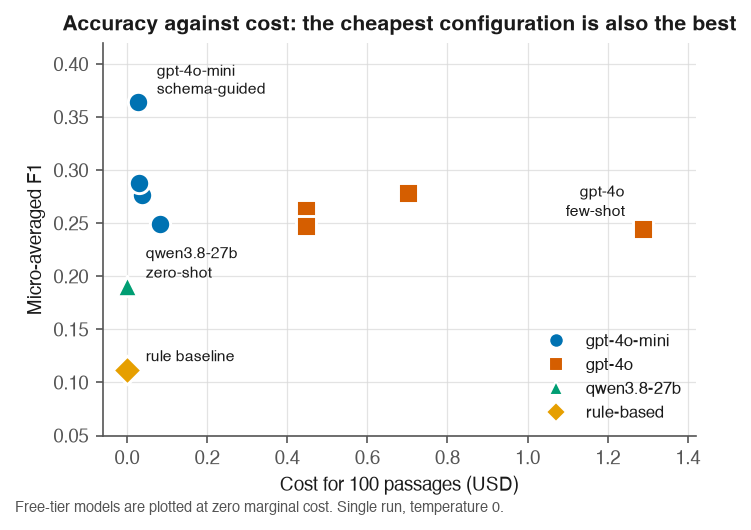
\includegraphics[width=\linewidth]{figures/fig1_cost_vs_f1.pdf}
\caption{Accuracy against cost. The relationship is the finding: the strongest configuration sits at the far left, and the most expensive configuration scores lower than one costing a forty-seventh as much. Free-tier models are plotted at zero marginal cost. Marker shape encodes model family in addition to colour, so the figure survives greyscale reproduction.}
\label{fig:fig1_cost_vs_f1}
\end{figure}

F1 collapses precision and recall into one number, which hides whether a configuration is cautious or scattergun. Plotting the two axes separately against iso-F1 contours makes that visible:


\begin{figure}[H]
\centering
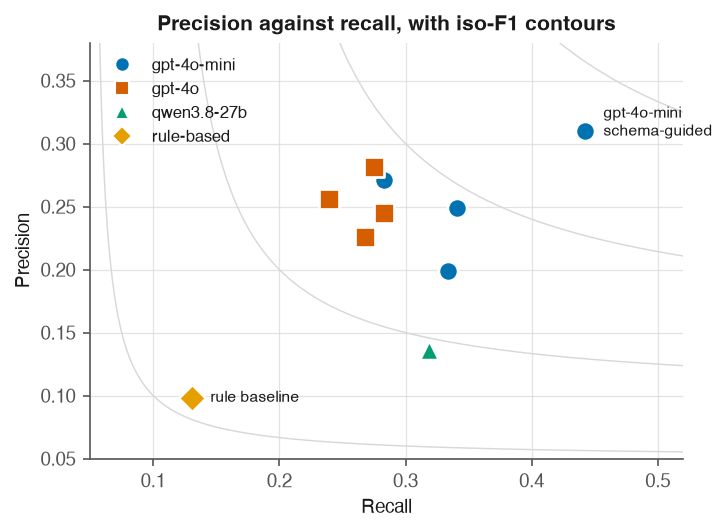
\includegraphics[width=\linewidth]{figures/fig4_precision_recall.pdf}
\caption{Precision against recall. Every language-model configuration sits above and to the right of the rule baseline on both axes, not only on the combined score. Recall varies more across the ten configurations than precision does, which is the more actionable observation for anyone tuning a prompt: the strategies mostly differ in how much they find, less in how often what they find is right.}
\label{fig:fig4_precision_recall}
\end{figure}

\section{Per-field results (RQ1)}

For the strongest configuration, gpt-4o-mini with schema-guided prompting:

\begin{center}
\small
\begin{tabular}{@{}lrrrrrrr@{}}
\toprule
\textbf{Field} & \textbf{P} & \textbf{R} & \textbf{F1} & \textbf{TP} & \textbf{FP} & \textbf{FN} & \textbf{Support} \\
\midrule
USES\_LINKER & 0.615 & 0.533 & 0.571 & 16 & 10 & 14 & 30 \\
USES\_PRECURSOR & 0.553 & 0.538 & 0.545 & 21 & 17 & 18 & 39 \\
IN\_SOLVENT & 0.485 & 0.471 & 0.478 & 16 & 17 & 18 & 34 \\
AT\_CONDITION & 0.140 & 0.206 & 0.167 & 7 & 43 & 27 & 34 \\
\bottomrule
\end{tabular}
\end{center}
Support counts are printed beside every score deliberately. SYNTHESIZED\_BY has a support of 1 and HAS\_PROPERTY, MEASURED\_AT and USED\_IN have a support of 0, so no conclusion is drawn about them; where a model emits triples for those relations they appear only as false positives, which is why HAS\_PROPERTY shows 21 false positives against zero support.

Excluding AT\_CONDITION, whose behaviour is explained in Section 5.5, the best configuration averages approximately 0.53 across the three remaining fields.


\begin{figure}[H]
\centering
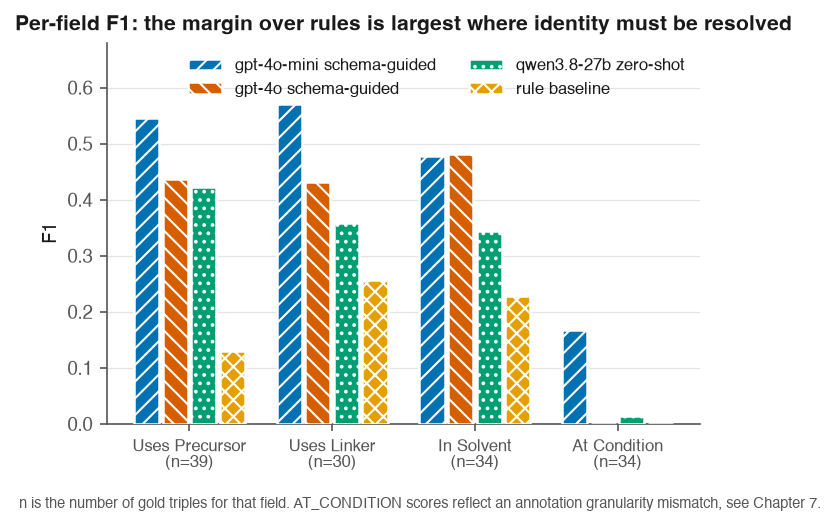
\includegraphics[width=\linewidth]{figures/fig2_per_field_f1.pdf}
\caption{Per-field F1 for four representative configurations, with the number of gold triples printed on each axis label. Support is shown in the figure rather than only in the caption so that fields backed by different amounts of evidence are not compared silently.}
\label{fig:fig2_per_field_f1}
\end{figure}

\section{Prompting strategies (RQ2) and open weight against commercial (RQ4)}

\textbf{Prompting strategies}, commercial models, all four strategies complete:

\begin{center}
\small
\begin{tabular}{@{}lrrrr@{}}
\toprule
\textbf{Model} & \textbf{zero-shot} & \textbf{few-shot} & \textbf{schema-guided} & \textbf{chain-of-thought} \\
\midrule
gpt-4o-mini & 0.287 & 0.249 & \textbf{0.364} & 0.277 \\
gpt-4o & 0.247 & 0.245 & 0.263 & \textbf{0.278} \\
\bottomrule
\end{tabular}
\end{center}
Schema-guided prompting wins clearly on the stronger configuration, supporting the premise that constraining output to the ontology helps. It does not win universally: on gpt-4o, chain-of-thought leads by 0.015, a margin a 138-triple gold standard cannot resolve. The defensible claim is that schema-guided is the best single choice observed, not that it dominates.

Few-shot is the weakest strategy on both models despite having by far the most expensive prompt, 4,054 template tokens against 652 for schema-guided. The worked examples cost roughly six times more per call and bought nothing measurable here.


\begin{figure}[H]
\centering
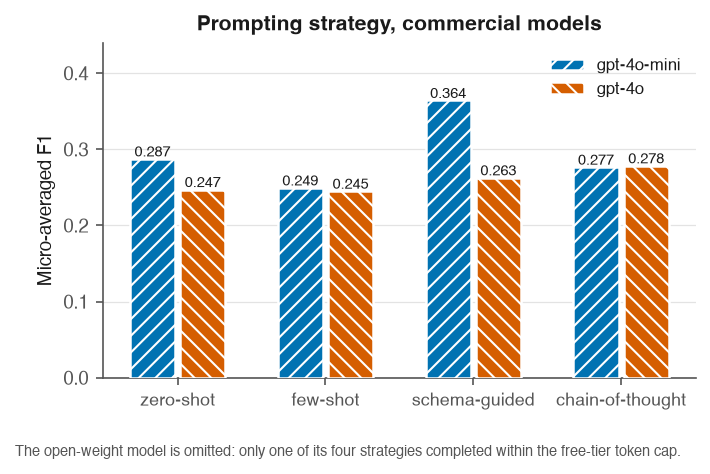
\includegraphics[width=\linewidth]{figures/fig3_prompting_strategies.pdf}
\caption{Prompting strategy by model. Only the two commercial models appear: just one of the open-weight model's four strategies completed within the free-tier token cap, and placing a single point beside two complete sets would invite a comparison the data cannot support.}
\label{fig:fig3_prompting_strategies}
\end{figure}

\textbf{Open weight against commercial}, compared like for like on zero-shot, the one strategy where all three models have complete coverage, so that model and strategy are not confounded:

\begin{center}
\small
\begin{tabularx}{\linewidth}{@{}Xrrr@{}}
\toprule
\textbf{Model} & \textbf{F1} & \textbf{Cost (USD)} & \textbf{Mean latency} \\
\midrule
gpt-4o-mini (commercial) & 0.287 & 0.030 & 3.8 s \\
gpt-4o (commercial) & 0.247 & 0.447 & 3.2 s \\
qwen3.8-27b (open weight) & 0.191 & 0.000 & 13.2 s \\
rule-based baseline & 0.112 & 0.000 & 0.001 s \\
\bottomrule
\end{tabularx}
\end{center}
The ordering is commercial, then open weight, then rules. The open-weight model reaches approximately two thirds of the best commercial F1 at zero marginal cost and roughly four times the latency, the latter being a property of the free serving tier rather than of the model.

\textbf{The cheaper commercial model outperforms the more expensive one.} gpt-4o-mini beats gpt-4o on three of four prompting strategies. The strongest configuration overall costs 0.028 USD; the most expensive configuration, gpt-4o few-shot, costs 1.289 USD and scores lower, a 47-fold cost difference in favour of the weaker model. Chapter 6 discusses the likely mechanism.

\section{Knowledge graph (RQ5)}

Loading the rule-based extractions over all 794 synthesis passages produced a graph of \textbf{485 distinct nodes and 2,429 relationships across 182 papers}, from 1,864 triples with zero skipped and zero load errors. Entity resolution collapses 3,728 node merge operations into 485 distinct nodes.

\textbf{Provenance is verified rather than asserted.} The \texttt{provenance\_violations} query, which returns any entity lacking a MENTIONED\_IN edge to a source paper, returns zero rows.

Cross-paper aggregation over synthesis methods:

\begin{center}
\small
\begin{tabularx}{\linewidth}{@{}Xrr@{}}
\toprule
\textbf{Method} & \textbf{Papers} & \textbf{MOFs} \\
\midrule
solvothermal & 61 & 30 \\
hydrothermal & 43 & 12 \\
electrochemical & 36 & 6 \\
microwave-assisted & 36 & 6 \\
stirred at room temperature & 35 & 5 \\
reflux & 21 & 3 \\
\bottomrule
\end{tabularx}
\end{center}
DigiMOF reported more hydrothermal (5,677) than solvothermal (3,672) records and described that ordering as surprising, since solvothermal is the more common laboratory route. This corpus shows the opposite ordering. The difference may reflect corpus composition, an open-access Europe PMC set against a CSD-derived one, or a difference in how each system infers an unnamed route. It is recorded here as an open question rather than resolved.

\section{What is not reported, and why}

Three of four open-weight prompting strategies could not be completed. The free serving tier caps this model at 200,000 tokens per day and 8,000 per minute. The per-minute throttle is handled by retrying on the provider's stated delay; the daily cap is a hard stop. Schema-guided completed 26 of 100 passages before exhaustion and few-shot completed 3 of 100.

Both were deleted from the results rather than scored. A configuration answering 26 of 100 passages is still scored against all 138 gold triples and reports an artificially low recall, which would misrepresent a rate-limited model as a weak one. Reporting a strategy as not obtained is honest; reporting it as scoring near zero is not.

RQ4 therefore rests on a single prompting strategy for the open-weight side.

\section{DigiMOF and SynMOF agreement (RQ3)}

RQ3 asked where and why LLM extractions disagree with the DigiMOF and SynMOF reference databases. This section reports what could be established and, more importantly, what could not. Every number below is produced by \texttt{python -m src.evaluation.build\_reference\_join} followed by \texttt{python -m src.evaluation.agreement\_analysis}, which rebuild the join from the two published source files rather than from a stored intermediate.

\textbf{The two databases were joined on CSD refcode.} DigiMOF's Supporting Information Master sheet holds 24,785 rows covering 24,732 distinct refcodes, and the manually curated SynMOF subset holds 840. Both sides are deduplicated on refcode before joining, because DigiMOF repeats some refcodes and an undeduplicated join returns 513 rows for the same materials. The intersection is \textbf{509 distinct MOFs}.

Field coverage within that intersection:

\begin{center}
\small
\begin{tabularx}{\linewidth}{@{}lrX@{}}
\toprule
\textbf{Field} & \textbf{Source} & \textbf{Coverage} \\
\midrule
Topology & DigiMOF & 509/509 (100 percent) \\
Temperature & SynMOF & 509/509 (100 percent) \\
Time & SynMOF & 509/509 (100 percent) \\
Primary metal & SynMOF & 509/509 (100 percent) \\
Metal & DigiMOF & 494/509 (97 percent) \\
Yield & SynMOF & 374/509 (74 percent) \\
Linker & DigiMOF & 159/509 (31 percent) \\
\bottomrule
\end{tabularx}
\end{center}
The linker coverage of 31 percent is the notable figure: the field this study cares most about is the one the reference databases are least complete on.

The intersection is dominated by water (351 records) and DMF (217), with a median synthesis temperature of 120 °C and a median reaction time of 72 hours. The leading metals are Cu (109), Zn (100), Cd (68) and Co (60).

\textbf{Agreement between the two databases.} Where both name a metal, they agree on \textbf{468 of 473 comparable records, 98.9 percent}. Agreement is defined as SynMOF's single primary metal appearing among the metals DigiMOF lists, since DigiMOF concatenates the metals of a bimetallic framework into one string. A further 36 records are not comparable because DigiMOF's metal field is empty or holds the literal value 0; these are excluded rather than counted as disagreements. The five genuine conflicts are substantive rather than cosmetic, for example refcode HUNBIB, recorded as Fe by DigiMOF and As by SynMOF.

\textbf{Why RQ3 cannot be answered as posed.} Both reference databases are keyed by CSD refcode. The gold standard is keyed by the MOF name as the paper writes it. Joining the two requires a name-to-refcode resource this project does not have, which is the same obstacle recorded in Section 7.7. The refcode-level overlap between the gold standard and the intersection is therefore \textbf{undetermined}, and no per-record agreement rate against DigiMOF or SynMOF can be computed.

What can be computed without that resource is a weaker screen. Of the 33 distinct MOF names in the gold standard, 9 have a composition, a metal and a linker, settled enough in the literature to write down; the remaining 24 do not, because a label such as "Ce-MOF" or a bare "COF" names no specific composition. Of those 9, \textbf{one has its composition present in the intersection}: Cu\textsubscript{3}(BTC)\textsubscript{2}, which is HKUST-1, matches refcode REYMOZ (Cu, 1,3,5-benzenetricarboxylic acid, tbo topology).

That single match is reported with its limits attached. A shared composition is a necessary but not a sufficient condition for identity, because the same metal and linker can assemble into different frameworks carrying different refcodes. It is enough to show that the gold standard and the reference intersection are not disjoint, and not enough to confirm any individual MOF as the same material. RQ3 is therefore recorded as unanswered, and the reasons are stated in Section 7.7 rather than presented as a result.


\chapter{Discussion}


I want to use this chapter to actually think through the results in Chapter 5, rather than restate them with different wording. Three questions seem worth answering properly: what the pre-registered prediction actually tells me, why the cheaper model beat the more expensive one, and what the rule baseline's weak MOF-identification rate says about maintaining a system like it. I will end by coming back to the gap I set out in Chapter 2 and being honest about how much of it this project actually closes.

\section{What the pre-registered prediction confirms, and what it does not}

I recorded a prediction before running a single model: the margin over the rule baseline should be largest on USES\_PRECURSOR and USES\_LINKER, and smallest on AT\_CONDITION and IN\_SOLVENT. The reasoning was that naming the material scattered across a passage takes something closer to reading comprehension, while matching a condition or a solvent is closer to pattern spotting. The measured ordering matched that exactly (Section 5.1), and I think it is fair to call that a real confirmation, not a pattern I noticed after the fact and then described as expected.

I still want to be careful about what it establishes. It tells me \emph{where} the gap between rules and language models is largest, and the reasoning I used to predict that turned out to point the right way. It does not tell me \emph{why} in any mechanistic sense. I never looked at what happens inside the model, only at what came out the other end, so a prediction holding up is evidence the reasoning is \emph{consistent} with the result, not proof that the reasoning is the actual explanation.

Sitting with the numbers a bit longer, I think the result also sharpens something the DigiMOF authors said rather than just testing it. They wrote that implicit synthesis routes, ones a paper implies through solvent and temperature instead of naming outright, are "challenging to extract using rule-based NLP" (Glasby et al., 2023), which is a claim about \emph{inferring a method}. What I found is a step earlier and, honestly, more basic: the rule baseline's biggest problem is not inferring the method, it is knowing which MOF the passage is even about in the first place (Section 6.3). I do not think these two findings contradict each other. A system that cannot name the product of a synthesis has little chance of correctly inferring its method from indirect cues either, since five of the eight relations in this ontology, and probably DigiMOF's extraction logic too, hang off the MOF node. I tested the prediction relation by relation, but the MOF-identification finding is, I think, a good part of the reason the rule baseline's disadvantage shows up everywhere rather than only on the fields that need inference.

\section{Why the cheaper model outperformed the more expensive one}

This is the finding I am least able to fully explain, and also the one I think matters most practically. gpt-4o-mini beat gpt-4o on three of the four prompting strategies, at roughly a forty-seven-fold difference in cost. Before I try to explain it, two things about how I measured it matter.

First, F1 against a fixed gold standard punishes a missed triple and a wrong triple the same way. A model that reports more candidate triples per passage does not automatically gain recall from that, and it will lose precision if a meaningful share of those extra triples are wrong. Second, looking at the per-field breakdown in Section 5.3, gpt-4o-mini's advantage sits mostly in USES\_PRECURSOR and USES\_LINKER, which happen to be the two fields with the most gold support (39 and 30 triples) and the two where the rule baseline already trailed the most. That is exactly where the two commercial models had the most room in the data to be told apart.

My best guess, and I want to be clear it is a guess rather than something I have verified, is that gpt-4o's answers are simply more elaborate. It seems to surface more candidate entities per passage, including plausible-sounding ones that were not actually part of the specific synthesis being described, a reagent mentioned in passing rather than one used in the recipe. Against a strict matcher and a gold standard of only 138 triples, that kind of verbosity turns into false positives rather than extra correct answers. That story is consistent with the precision figures in Section 5.2, where gpt-4o's precision is not obviously better than gpt-4o-mini's despite doing better on most general benchmarks, but consistency is not the same as confirmation. I have listed a manual error review, actually reading the false positives from both models side by side, as the next concrete step in Chapter 8, because that is the only way I can think of to test this properly rather than just gesture at it. Until that is done, the honest claim is the narrower one already in Chapter 5: the cheaper model wins on this evaluation at this cost, and the reason why is a hypothesis, not a result.

There is a plainer possible explanation too, and I do not want to quietly favour the more interesting story over it. gpt-4o-mini might just be better suited to a concise, schema-constrained extraction task, independent of any verbosity effect at all. Either way, the practical takeaway is the same. Whatever a model's reputation on general benchmarks, it did not predict how it would do on this specific task, and if this study had only tested the larger flagship model of each vendor, on the assumption that bigger is safer, it would have reached the wrong conclusion for no better reason than not having checked.

\section{What the 15 percent MOF-identification rate means for rule-based pipeline maintainers}

The rule baseline names a MOF in only 121 of the 794 synthesis passages in the full corpus, about 15 percent (Section 8.3; reproducible with \texttt{python -m src.pipeline --extractors rule\_based --no-resume}). Figure 6 shows where the other 673 passages go. 331 name the MOF somewhere else in the paper, usually at first mention rather than in the synthesis paragraph itself, and 251 use a generic label like "compound 1" that only resolves to an actual chemical identity through a table or a cross-reference the passage itself does not contain. The remaining 91 are cases such as a name coined by the authors that no fixed dictionary could have anticipated.


\begin{figure}[H]
\centering
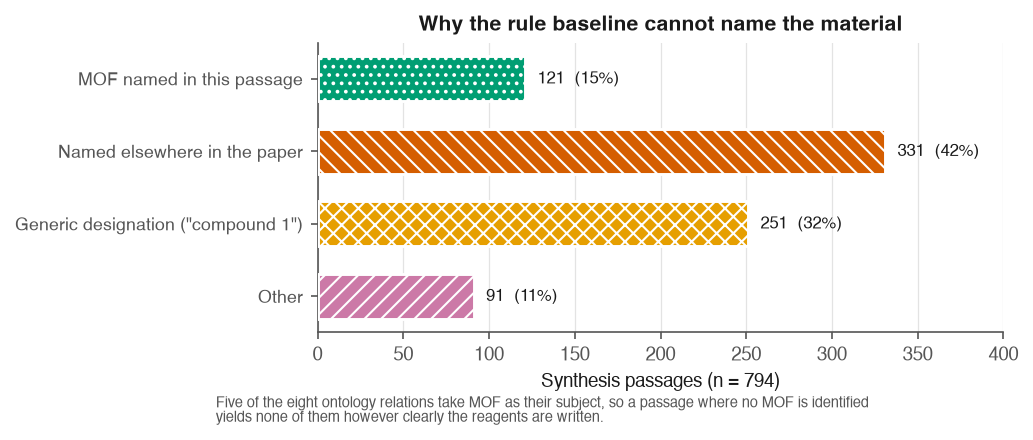
\includegraphics[width=\linewidth]{figures/fig6_baseline_failure_modes.pdf}
\caption{The rule baseline's dominant failure is not a missing dictionary entry. Coreference across a paper and generic numbered designations together account for more than four times as many passages as successful MOF identification.}
\label{fig:fig6_baseline_failure_modes}
\end{figure}

Neither of the two big causes is a lexicon gap. You can always grow a vocabulary, and DigiMOF's own parsers are already extensive, but no amount of vocabulary helps when the information the parser needs simply is not in the passage it is looking at. If I were maintaining or extending a rule-based pipeline over this kind of literature, I do not think I would reach for a bigger dictionary first. I would reach for coreference resolution across a paper, so a synthesis paragraph can be linked back to the name the compound was given when it was first introduced, and for table parsing, since a numbered designation is very often defined in a table that the running text never repeats. Both are engineering problems a rule-based system can solve without becoming a language model, and honestly both look more tractable to me than the implicit-route inference problem Glasby et al. (2023) describe, because neither requires inference. They just require linking two places in the same document that already state the fact plainly.

I read this as reframing rather than overturning the claim I set out to test in Chapter 2. Implicit method inference is a real difficulty for rule-based extraction, and the smaller LLM margins I measured on IN\_SOLVENT and AT\_CONDITION are consistent with rules already handling the easier, locally-patterned end of that spectrum reasonably well. But for MOF synthesis specifically, the bigger and more basic obstacle sits earlier in the pipeline, at working out which compound is even being discussed, and that is why the language model's advantage over rules in this study turned out larger on those identity-dependent fields than the original framing led me to expect.

\section{What this means for building such a pipeline today}

Two choices in this project were made for cost reasons, not as a deliberate research design, and both turned out to also be the ones the results actually support. Schema-guided prompting, the cheapest template I tested at 652 tokens against 4,054 for few-shot, was also the best-performing strategy on the strongest model. And the free-tier open-weight model, at zero marginal cost, reached about two thirds of the best commercial F1. Put together with the cheaper-model result in Section 6.2, the shape of this whole evaluation is that the most expensive choices I tested, few-shot prompting and the larger commercial model, were beaten by cheaper alternatives on every axis I measured. I do not think that means an expensive configuration is never worth it. It means that for this task, on this gold standard, it was not, and anyone building something similar on a tight budget now has an actual measurement to start from instead of an assumption.

The absolute numbers are still modest, and I do not want to end this chapter sounding more confident than they warrant. Chapter 7 sets out why 0.364 micro-F1, or roughly 0.53 once the field whose scores measure annotation granularity rather than extraction quality is excluded, is a lower bound rather than a ceiling, and what it would actually take to close the remaining gap to the target I set in the exposé.

\section{What the reference databases could and could not tell me}

I set out in Chapter 2 to validate extractions against DigiMOF and SynMOF, and that is the research question this project does not answer. It is worth being precise about why, because the reason is not that the analysis failed but that it was posed against the wrong key.

The two databases share 509 MOFs by CSD refcode, and on those they agree about the metal 98.9 percent of the time. I find that number genuinely useful, and not for the reason I expected. It says two independently built text-mining efforts, one rule-based over full text and one manually curated, converge almost completely on the metal when they describe the same material. That is a reassuring result about the reference databases themselves, and it sets a rough ceiling on what agreement between any two extraction systems ought to look like on a field this well defined.

The obstacle is the key. DigiMOF and SynMOF are indexed by CSD refcode, and my gold standard is indexed by whatever name the paper used. Getting from "MOF-303" to a refcode needs a mapping resource I do not have, so I cannot compute the overlap, and I want to say plainly that undetermined is not the same as zero. An earlier draft of this chapter asserted that the overlap was zero and that the corpus contained no classic MOFs. Both claims were wrong. The gold standard contains ZIF-8, MIL-101(Cr), UiO-66-NH\textsubscript{2}, NU-1000 and Cu\textsubscript{3}(BTC)\textsubscript{2}, and that last one is HKUST-1, whose composition sits in the intersection as refcode REYMOZ. I could only establish a composition-level match rather than a confirmed identity, since the same metal and linker can build different frameworks, but it is enough to rule out the disjointness I had claimed.

What I take from this is a lesson about evaluation design rather than about extraction. I chose the corpus for one property, open access with structured full text, and chose the reference databases for another, coverage of MOF synthesis. Nothing forced those two choices to share an identifier, and I did not check that they did until after the corpus was built and annotated. The 31 percent linker coverage inside the intersection points the same way: even had the join worked, the field I most wanted to validate is the field DigiMOF is thinnest on. An agreement study needs the join key and the field coverage settled before the corpus is collected, not after.

So RQ3 stays open, and Chapter 8 records what closing it would take. What I can offer in its place is narrower but real: the reference databases are highly self-consistent on the material they share, my corpus is not disjoint from them, and the specific reason a per-record comparison is out of reach is an identifier mismatch rather than anything about how well the models read a paper.


\chapter{Limitations and Threats to Validity}


This chapter states what the study cannot show. Several of these limitations were discovered during the work and are recorded with the evidence that produced them, so that a reader can judge their severity rather than take the assessment on trust.

\section{The AT\_CONDITION scores measure annotation granularity, not extraction quality}

AT\_CONDITION scores between 0.00 and 0.17 for every extractor, with 43 false positives for the best configuration. The cause is a granularity mismatch, not extraction failure. The annotator recorded a complete condition string as one value, for example "100 °C for 1 h, then additional 1 h", while the models emit one triple per condition, "100 °C" and "1 h" separately. Neither convention is wrong and the metric punishes the mismatch.

\textbf{Consequence.} No claim about condition-extraction accuracy in this study is trustworthy. The field is reported for completeness and excluded from conclusions. Excluding it, the best configuration averages approximately 0.53 across the three remaining fields.

\textbf{Remedy for future work.} Either fix the annotation convention to one condition per triple, or implement a set-valued comparison for this field that credits a decomposition of a combined gold value.

\section{Absolute scores are depressed by surface-form mismatch}

Manual inspection of gold against predicted triples shows correct extractions scored as failures because of surface form. Examples observed:

\begin{center}
\small
\begin{tabularx}{\linewidth}{@{}XXX@{}}
\toprule
\textbf{Gold} & \textbf{Predicted} & \textbf{Status} \\
\midrule
\texttt{ZrOCl\textsubscript{2}·8H\textsubscript{2}O} & \texttt{ZrOCl2·8H2O} & matched, the normaliser handles Unicode subscripts \\
\texttt{DMF} & \texttt{dimethylformamide (DMF)} & matched only after a fix, see 7.3 \\
\texttt{[emim]Br / bmim} & \texttt{1-ethyl-3-methylimidazolium bromide} & not matched, same reagent, absent from the synonym table \\
\bottomrule
\end{tabularx}
\end{center}
The measured F1 of 0.364 is therefore a lower bound on semantic extraction quality. A study with a chemical-name resolution service, for example one backed by PubChem or ChemSpider identifiers, would report higher numbers for identical extractions. This limits comparability with published figures obtained under different matching regimes.

\section{One normalisation change was made after seeing the data}

\texttt{normalize\_chemical} was extended to resolve "full name (ABBREV)" through either half after inspection of failures revealed the pattern. This is disclosed rather than folded in silently. The change raised every extractor by between 0.006 and 0.027, including the rule baseline, and both sets of numbers are preserved in the repository history. A uniform lift across all systems is consistent with a genuine surface-form fix rather than tuning toward a target, but the reader should know the change was made in response to the data.

\section{The gold standard is small, and smaller than planned}

The exposé specified 150 to 200 annotated passages; 100 were annotated, yielding 138 triples. The reduction was a deliberate response to a fixed submission date and the fact that the gold standard must be produced by hand. The consequence is wide confidence intervals on every per-field score and insufficient support for four of the eight relations. Differences of the order of 0.015, such as the schema-guided against chain-of-thought gap on gpt-4o, cannot be resolved at this sample size and are not treated as findings.

Single-annotator annotation is a further limitation: no inter-annotator agreement statistic can be computed, so the gold standard's own consistency is unmeasured.

\section{A defect in the annotation tool required an evaluation concession}

The annotation interface retained a text field's previous value when the relation changed while its label changed underneath. Consequently every IN\_SOLVENT and AT\_CONDITION gold triple, 68 of 138, records the MOF's name in the subject position where the synthesis method belongs. The tool was fixed, but the recorded gold standard carries the artefact.

The evaluation therefore scores those two relations on the object alone. This is independently defensible, because the ontology routes solvents and conditions through a method that acts as a connector rather than a claim, but it means the study cannot show whether a model attaches a solvent to the correct synthesis when a passage describes several. Correcting the gold subjects with a model was rejected, since generating ground truth with a language model would make the evaluation circular.

\section{The open-weight comparison rests on one prompting strategy}

Free-tier token caps prevented three of four open-weight strategies from completing. RQ4 is therefore answered on zero-shot only. The comparison is like for like, since all three models have complete zero-shot coverage, but it cannot show whether the open-weight model responds to prompting strategy in the same way the commercial models do.

The exposé specified Llama-3 via a local Ollama installation. That plan was abandoned twice: first because 8 GB of RAM made several thousand local inferences impractical within the schedule, and then because the chosen hosted provider had retired every Llama chat model by the time of the run. The substitute, qwen3.8-27b, is genuinely open-weight and independent of the commercial models' lineage, but it is not the model the exposé named.

\section{Corpus scope and its effect on RQ3}

The corpus is restricted to the Europe PMC open-access subset. Much open-access chemistry is not indexed there, so the corpus is not a random sample of MOF literature. The publisher distribution does overlap DigiMOF's sources, which supports the feasibility of the agreement analysis, but coverage bias remains.

The DigiMOF supporting information is keyed by CSD refcode while this corpus is keyed by DOI and the gold standard by the MOF name a paper uses. A per-record join requires a name-or-DOI-to-refcode mapping that is normally obtained from a licensed resource. Section 5.7 reports what could be established without one: the two reference databases were joined to each other on refcode, giving 509 shared MOFs on which they agree about the metal 98.9 percent of the time, and a composition-level screen shows the gold standard is not disjoint from that intersection. What could not be established is any per-record agreement rate between this study's extractions and either database.

\textbf{Consequence.} RQ3 is not answered in this report. The overlap between the gold standard and the reference intersection is undetermined rather than zero, a distinction this report draws deliberately, since an earlier draft asserted zero and was wrong. A further constraint would bind even if the mapping were obtained: DigiMOF records a linker for only 31 percent of the shared MOFs, so the field this study most wants to validate is the one the reference is thinnest on.

\section{Single run, no variance estimate}

Every configuration was run once, at temperature 0. No variance across repeated runs is reported, so apparent differences between configurations include an unmeasured sampling component even at temperature 0, where provider-side non-determinism can still occur.


\chapter{Conclusion and Outlook}


\section{What was built}

An end-to-end, reproducible pipeline that collects open-access MOF literature, segments it into synthesis passages, extracts structured synthesis records with either a rule-based system or a language model under four prompting strategies, evaluates those extractions per field against a hand-annotated gold standard, and loads them into a Neo4j knowledge graph in which every entity is traceable to the sentence that produced it. Provenance completeness is verified by query rather than asserted.

\section{What was found}

\textbf{Language models beat the rule-based baseline on every configuration tested}, and they beat it by the largest margin exactly where a pre-registered prediction said they would: on identifying which material is being made and from what. The margin is +0.42 F1 on metal precursors and +0.31 on organic linkers, falling to +0.25 on solvents and +0.17 on conditions, which are the fields local surface patterns already handle.

\textbf{The cheaper commercial model outperformed the more expensive one} on three of four prompting strategies, at a 47-fold cost difference in favour of the cheaper model. The most likely mechanism, that a larger model produces more elaborate output and therefore more false positives against a fixed gold standard, is consistent with the precision figures but is not established here.

\textbf{Schema-guided prompting was the best single choice observed}, though not universally, and few-shot prompting was the weakest strategy on both commercial models despite the most expensive prompt by a factor of six.

\textbf{The open-weight model reached approximately two thirds of the best commercial F1 at zero marginal cost.} For a pipeline that must be reproducible without an institutional budget, that is a meaningful result rather than a shortfall.

\textbf{Absolute accuracy is well below the target stated in the exposé.} The best configuration reaches 0.364 micro-F1 against a target of 0.80. Chapter 7 sets out how much of that gap is attributable to surface-form matching and annotation granularity rather than extraction quality, and reports that the best configuration reaches approximately 0.53 when the field whose scores measure granularity is excluded.

\section{What this says about the field}

The DigiMOF authors observed that synthesis routes implied rather than named are hard for rule-based extraction. This work provides a quantified version of that observation from the other direction: the rule-based baseline identified a MOF in only 15 percent of synthesis passages, and because the ontology roots five relations at the MOF node, that single failure suppresses most of what a rule-based system could otherwise extract. Of the passages where no MOF was identified, 331 named it elsewhere in the same paper and 251 used a generic designation such as "compound 1". Those are not lexicon gaps that a larger dictionary would close.

\section{Future work}

\begin{enumerate}
\item \textbf{Complete RQ3.} The blocker is an identifier mismatch, not a missing analysis: the reference databases are keyed by CSD refcode and this corpus by DOI and MOF name. Obtain a name-or-DOI-to-refcode mapping, then run the per-record comparison that Section 5.7 sets up but cannot execute. Note that DigiMOF carries a linker for only 31 percent of the shared MOFs, so linker agreement will rest on a small subset even then.
\item \textbf{Complete the open-weight strategy sweep}, which requires either a paid serving tier or several days of free-tier quota.
\item \textbf{Repair the condition evaluation}, either by changing the annotation convention to one condition per triple or by implementing set-valued comparison for that field.
\item \textbf{Add chemical identifier resolution} so that surface-form variation stops being scored as extraction error.
\item \textbf{Enlarge the gold standard and add a second annotator}, which would both narrow the confidence intervals and allow an inter-annotator agreement statistic.
\item \textbf{Investigate the cheap-model result} with a manual error review, since it is the most practically consequential finding here and currently rests on an unverified mechanism.
\end{enumerate}


\chapter{References}


Every entry below was verified against a live bibliographic source (Crossref, OpenAlex or arXiv) rather than written from memory. The load-bearing citations were re-verified on 2026-09-01. Formatting follows APA 7.

Ansari, M., \& Moosavi, S. M. (2024). Agent-based learning of materials datasets from the scientific literature. \emph{Digital Discovery, 3}, 2607-2617. \href{https://doi.org/10.1039/D4DD00252K}{https://doi.org/10.1039/D4DD00252K}

Bae, S., Jeon, M., Moon, H., et al. (2025). Text mining in MOF research: From manual curation to large language model-based automation. \emph{Chemical Communications, 61}, 11083-11094. \href{https://doi.org/10.1039/D5CC02511G}{https://doi.org/10.1039/D5CC02511G}

Bai, X., He, S., Li, Y., Xie, Y., Zhang, X., Du, W., \& Li, J. (2025). Construction of a knowledge graph for framework material enabled by large language models and its application. \emph{npj Computational Materials, 11}, 51. \href{https://doi.org/10.1038/s41524-025-01540-6}{https://doi.org/10.1038/s41524-025-01540-6}

Chung, Y. G., Haldoupis, E., Bucior, B. J., et al. (2019). Advances, updates, and analytics for the computation-ready, experimental metal-organic framework database: CoRE MOF 2019. \emph{Journal of Chemical \& Engineering Data, 64}(12), 5985-5998. \href{https://doi.org/10.1021/acs.jced.9b00835}{https://doi.org/10.1021/acs.jced.9b00835}

Dagdelen, J., Dunn, A., Lee, S., Walker, N., Rosen, A. S., Ceder, G., Persson, K. A., \& Jain, A. (2024). Structured information extraction from scientific text with large language models. \emph{Nature Communications, 15}, 1418. \href{https://doi.org/10.1038/s41467-024-45563-x}{https://doi.org/10.1038/s41467-024-45563-x}

Dreger, M., Malek, K., \& Eikerling, M. (2025). Large language models for knowledge graph extraction from tables in materials science. \emph{Digital Discovery, 4}, 1221-1231. \href{https://doi.org/10.1039/D4DD00362D}{https://doi.org/10.1039/D4DD00362D}

Edge, D., Trinh, H., Cheng, N., Bradley, J., Chao, A., Mody, A., Truitt, S., \& Larson, J. (2024). From local to global: A GraphRAG approach to query-focused summarization. arXiv:2404.16130. \href{https://arxiv.org/abs/2404.16130}{https://arxiv.org/abs/2404.16130}

Glasby, L. T., Gubsch, K., Bence, R., Oktavian, R., Isoko, K., Moosavi, S. M., Cordiner, J. L., Cole, J. C., \& Moghadam, P. Z. (2023). DigiMOF: A database of metal-organic framework synthesis information generated via text mining. \emph{Chemistry of Materials, 35}(11), 4510-4524. \href{https://doi.org/10.1021/acs.chemmater.3c00788}{https://doi.org/10.1021/acs.chemmater.3c00788}

Gupta, T., Zaki, M., Krishnan, N. M. A., \& Mausam. (2022). MatSciBERT: A materials domain language model for text mining and information extraction. \emph{npj Computational Materials, 8}, 102. \href{https://doi.org/10.1038/s41524-022-00784-w}{https://doi.org/10.1038/s41524-022-00784-w}

Jablonka, K. M., Schwaller, P., Ortega-Guerrero, A., \& Smit, B. (2024). Leveraging large language models for predictive chemistry. \emph{Nature Machine Intelligence, 6}, 161-169. \href{https://doi.org/10.1038/s42256-023-00788-1}{https://doi.org/10.1038/s42256-023-00788-1}

Jalali, M., Wonanke, A. D. D., \& Wöll, C. (2023). MOFGalaxyNet: A social network analysis for predicting guest accessibility in metal-organic frameworks utilizing graph convolutional networks. \emph{Journal of Cheminformatics, 15}, 94. \href{https://doi.org/10.1186/s13321-023-00764-2}{https://doi.org/10.1186/s13321-023-00764-2}

Kim, E., Huang, K., Saunders, A., McCallum, A., Ceder, G., \& Olivetti, E. (2017). Materials synthesis insights from scientific literature via text extraction and machine learning. \emph{Chemistry of Materials, 29}(21), 9436-9444. \href{https://doi.org/10.1021/acs.chemmater.7b03500}{https://doi.org/10.1021/acs.chemmater.7b03500}

Kononova, O., Huo, H., He, T., Rong, Z., Botari, T., Sun, W., Tshitoyan, V., \& Ceder, G. (2019). Text-mined dataset of inorganic materials synthesis recipes. \emph{Scientific Data, 6}, 203. \href{https://doi.org/10.1038/s41597-019-0224-1}{https://doi.org/10.1038/s41597-019-0224-1}

Lewis, P., Perez, E., Piktus, A., et al. (2020). Retrieval-augmented generation for knowledge-intensive NLP tasks. \emph{Advances in Neural Information Processing Systems, 33}. arXiv:2005.11401. \href{https://arxiv.org/abs/2005.11401}{https://arxiv.org/abs/2005.11401}

Lin, Z., Ren, D., Ran, K., et al. (2025). Reshaping MOFs text mining with a dynamic multi-agent framework of large language models. arXiv:2504.18880. \href{https://arxiv.org/abs/2504.18880}{https://arxiv.org/abs/2504.18880}

Luo, Y., Bag, S., Zaremba, O., Cierpka, A., Andreo, J., Wuttke, S., Friederich, P., \& Tsotsalas, M. (2022). MOF synthesis prediction enabled by automatic data mining and machine learning. \emph{Angewandte Chemie International Edition, 61}, e202200242. \href{https://doi.org/10.1002/anie.202200242}{https://doi.org/10.1002/anie.202200242}

Olivetti, E., Cole, J., Kim, E., Kononova, O., Ceder, G., Han, T., \& Hiszpanski, A. (2020). Data-driven materials research enabled by natural language processing and information extraction. \emph{Applied Physics Reviews, 7}, 041317. \href{https://doi.org/10.1063/5.0021106}{https://doi.org/10.1063/5.0021106}

Pan, S., Luo, L., Wang, Y., Chen, C., Wang, J., \& Wu, X. (2024). Unifying large language models and knowledge graphs: A roadmap. \emph{IEEE Transactions on Knowledge and Data Engineering, 36}(7), 3580-3599. \href{https://doi.org/10.1109/TKDE.2024.3352100}{https://doi.org/10.1109/TKDE.2024.3352100}

Polak, M. P., \& Morgan, D. (2024). Extracting accurate materials data from research papers with conversational language models and prompt engineering. \emph{Nature Communications, 15}, 1569. \href{https://doi.org/10.1038/s41467-024-45914-8}{https://doi.org/10.1038/s41467-024-45914-8}

Shi, L., Liu, Z., Yang, Y., et al. (2024). LLM-based MOFs synthesis condition extraction using few-shot demonstrations. arXiv:2408.04665. \href{https://arxiv.org/abs/2408.04665}{https://arxiv.org/abs/2408.04665}

Swain, M. C., \& Cole, J. M. (2016). ChemDataExtractor: A toolkit for automated extraction of chemical information from the scientific literature. \emph{Journal of Chemical Information and Modeling, 56}(10), 1894-1904. \href{https://doi.org/10.1021/acs.jcim.6b00207}{https://doi.org/10.1021/acs.jcim.6b00207}

Trewartha, A., Walker, N., Huo, H., Lee, S., Cruse, K., Dagdelen, J., Dunn, A., Persson, K. A., Ceder, G., \& Jain, A. (2022). Quantifying the advantage of domain-specific pre-training on named entity recognition tasks in materials science. \emph{Patterns, 3}(4), 100488. \href{https://doi.org/10.1016/j.patter.2022.100488}{https://doi.org/10.1016/j.patter.2022.100488}

Tshitoyan, V., Dagdelen, J., Weston, L., Dunn, A., Rong, Z., Kononova, O., Persson, K. A., Ceder, G., \& Jain, A. (2019). Unsupervised word embeddings capture latent knowledge from materials science literature. \emph{Nature, 571}, 95-98. \href{https://doi.org/10.1038/s41586-019-1335-8}{https://doi.org/10.1038/s41586-019-1335-8}

Wei, X., Cui, X., Cheng, N., et al. (2023). Zero-shot information extraction via chatting with ChatGPT. arXiv:2302.10205. \href{https://arxiv.org/abs/2302.10205}{https://arxiv.org/abs/2302.10205}

Weston, L., Tshitoyan, V., Dagdelen, J., Kononova, O., Trewartha, A., Persson, K. A., Ceder, G., \& Jain, A. (2019). Named entity recognition and normalization applied to large-scale information extraction from the materials science literature. \emph{Journal of Chemical Information and Modeling, 59}(9), 3692-3702. \href{https://doi.org/10.1021/acs.jcim.9b00470}{https://doi.org/10.1021/acs.jcim.9b00470}

Yang, W., Liu, Z., Tan, T., \& Hu, X. (2026). AgentCAT: An LLM agent for extracting and analyzing catalytic reaction data from chemical engineering literature. arXiv:2602.18479. \href{https://arxiv.org/abs/2602.18479}{https://arxiv.org/abs/2602.18479}

Ye, Y., Ren, J., Wang, S., \& Wan, Y. (2024). Construction and application of materials knowledge graph in multidisciplinary materials science via large language model. \emph{Advances in Neural Information Processing Systems, 37}. arXiv:2404.03080. \href{https://arxiv.org/abs/2404.03080}{https://arxiv.org/abs/2404.03080}

Yoshitake, M., \& Nagata, T. (2025). A method for LLM-based construction of a materials property knowledge graph: A case study. \emph{Applied Sciences, 15}(19), 10511. \href{https://doi.org/10.3390/app151910511}{https://doi.org/10.3390/app151910511}

Zaki, M., Jayadeva, Mausam, \& Krishnan, N. M. A. (2024). MaScQA: Investigating materials science knowledge of large language models. \emph{Digital Discovery, 3}, 313-327. \href{https://doi.org/10.1039/D3DD00188A}{https://doi.org/10.1039/D3DD00188A}

Zheng, Z., Zhang, O., Borgs, C., Chayes, J. T., \& Yaghi, O. M. (2023). ChatGPT chemistry assistant for text mining and the prediction of MOF synthesis. \emph{Journal of the American Chemical Society, 145}(32), 18048-18062. \href{https://doi.org/10.1021/jacs.3c05819}{https://doi.org/10.1021/jacs.3c05819}

\end{document}
